%% Template for SDP report, adapted from mlp_cw2_template, 2018. 

%% Based on  LaTeX template for ICML 2017 - example_paper.tex at 
%%  https://2017.icml.cc/Conferences/2017/StyleAuthorInstructions

\documentclass{article}
\usepackage[T1]{fontenc}
\usepackage{amssymb,amsmath}
\usepackage{txfonts}
\usepackage{microtype}
\usepackage{xspace}
\xspaceaddexceptions{\%}

% Lists with less spacing between items
\usepackage{paralist}

% For figures
\usepackage{graphicx}
\usepackage{subfig} 

% For citations
\usepackage{natbib}

% For algorithms
\usepackage{algorithm}
\usepackage{algorithmic}

% the hyperref package is used to produce hyperlinks in the
% resulting PDF.  If this breaks your system, please commend out the
% following usepackage line and replace \usepackage{mlp2017} with
% \usepackage[nohyperref]{mlp2017} below.
\usepackage{hyperref}
\usepackage{url}
\urlstyle{same}

% Packages hyperref and algorithmic misbehave sometimes.  We can fix
% this with the following command.
\newcommand{\theHalgorithm}{\arabic{algorithm}}


% Set up MLP coursework style (based on ICML style)
\usepackage{mlp2018}
\mlptitlerunning{SDP Demo \demoNumber  Group (\groupNumber)}
\bibliographystyle{icml2017}


\DeclareMathOperator{\softmax}{softmax}
\DeclareMathOperator{\sigmoid}{sigmoid}
\DeclareMathOperator{\sgn}{sgn}
\DeclareMathOperator{\relu}{relu}
\DeclareMathOperator{\lrelu}{lrelu}
\DeclareMathOperator{\elu}{elu}
\DeclareMathOperator{\selu}{selu}
\DeclareMathOperator{\maxout}{maxout}






%% You probably do not need to change anything above this comment

%% REPLACE the details in the following commands with your details
\setGroupNumber{1}
\setGroupName{My Group}
\setProductName{My Product}
\setLogoFileName{figs/sdp_logo_placeholder.png}

\begin{document} 

\makeSDPTitle{Project Plan}

% Previous MLP Style Title Layout working. 
% \twocolumn[
    % \mlptitle{\productName: SDP Demo \demoNumber}
    % \centerline{Group \groupNumber: \groupName}
% ]

\begin{abstract} 
The abstract should first consist of one sentence describing the intended functionality of your system. It should be followed by a few sentences (100--200 words) summarising the main goals that will bring your project to a successful completion. This should give the reader a clear expectation of what will be achieved throughout the semester.
\end{abstract} 

\section*{Outline}
\label{sec:intro}
The project plan serves to guide you in two purposes:
\begin{enumerate}
\item Thinking as a group about what you envision your system as trying to achieve, in a way that should support future decision making.
\item Agreeing an initial outline of how you will approach your work, so everyone knows what to expect and can tell when the plan starts to drift.
\end{enumerate}
It should have each of the following sections, with contents designed to address the questions listed (not just a list of questions and answers). Suggested lengths are given as a rough guide, but if you feel that a particular aspect is more or less important in your case then you can stray from them. Overall, this should be no more than 9 pages, excluding bibliography and appendix.
You might find it easiest to split up responsibility for writing sections, but you should still aim to have the discussions about your answers as a group to build some shared consensus about the vision. You will also want someone confident with their written English to make a final editorial pass to make everything flow together.
Plans are not meant to be final, but they should be what you currently intend on doing, with acknowledgement of where more information might be needed or what decisions might be dependent on other outcomes.


\textit{note: You should delete this section (no outline required).}

\section{Pitch} 
A concise overview of the core idea of your system, aimed at convincing the reader it is worth doing. ($\simeq 250$  words)

\section{The team} 
What are the main skills of the people in your team? What sorts of things would they each ideally like to work on (one may wish to work on something new, rather than an existing skill)? What do they think they would struggle with? Do they have any other working preferences (such as wanting to skew work towards the start of semester) that the team should consider?  ($\simeq 500$  words)

\section{Users} 
Who is the primary user of your system (who is it assisting)? What is the need that it fulfills for them? How do you expect their core interaction with it to go? What other aspects of this user’s needs or context might be important constraining factors on your design?

Are there other users who are not the primary user (for example, family, carers, maintenance teams) who will also regularly interact with the system? What are their core needs? Is there any potential conflict between the needs or priorities of different user groups, or other stakeholders?
This should be a good basis for creating \href{https://www.atlassian.com/agile/project-management/user-stories}{User Stories}, though we are not requiring you to provide a full set of those here.
 ($\simeq 750$ words)

\section{Impact}
How do you expect this system to be deployed (is it sold to individuals, provided by a company as a service, etc)? What do you anticipate the potential wider social impacts of the technology to be?
 ($\simeq 500$ words)

\section{Outcomes}
What concrete functionality do you want your system to have? How do these link to the user needs you outlined? How are they prioritised? What is necessary and what is optional? What are the (ideally measurable) ways you would demonstrate that you have achieved this functionality?
 ($\simeq 500$ words)

\section{Tasks}
What subsystems/areas (that require different skills / could be worked on relatively independently) does your project break down into? What capabilities are those subsystems reliant on each other for? Beyond the actual construction of the system, what additional types of work will be required?
How is overall team effort expected to be split between tasks (e.g. rough percentages of time)? What is the prioritisation of tasks? How will they be assigned to team members? Are there any other time constraints on tasks?
For each demo day (at least), you should list your team’s goals. If you want to know how to define effective goals, try \href{https://www.mindtools.com/pages/article/smart-goals.htm}{SMART} goals.
You should put together a Gantt chart summarising the above information (Maximum 1 page).

Though you won’t have space for it here, we advise you to do a full task decomposition (into tasks taking a day or less) for the purpose of assigning and tracking work in more detail. It is helpful to know if things are routinely taking more/less time than expected so you can do something about it.
 ($\simeq 750$ words)

\section{Risks}
What are the main risks in your project plan? What are the consequences if those risks are realised? How can you reduce the impact? This can be either to reduce the chances of something happening, or a contingency plan that is in place for if it does.
 ($\simeq 500$ words)

\section*{Advice}
\textit{note: You should delete this section (no Advice section is required).}

\subsection*{How to get a good mark}

Very good project plans will:
\begin{itemize}
    \item Answer all of the questions provided
    \item Include supporting research
    \item Justify key decisions made
    \item Draw links and dependencies between the answers (for example, clearly linking intended outcomes to the user stories they support)
    \item Be clear about priorities
    \item 	Be written precisely enough that another team could start the project from it
    \item Have a plan flexible enough that you are not stuck on one path with no ability to adapt later
\end{itemize}

As always, excellence marks (70+) are primarily for going over and above what is expected of you.

\subsection*{Latex tips}

Don't forget to replace the placeholders for your name, product, team logo and group number in the template.

You can include references to scientific papers \cite{langley00} or studies that will help justifying the value / interest of your system or validate a specific design choice.

You can summarize the tasks /risks in a table, (for instance, table~\ref{tab:sample-table}, using the \verb+table+ environment).

\begin{table*}[h]
\vskip 3mm
\begin{center}
\begin{small}
\begin{sc}
\begin{tabular}{lcccr}
\hline
\abovespace\belowspace
Task Name & Milestone  & Estimated time & Dependency &  Rough description \\
\hline
\abovespace
Task 1 & Milestone 1    & 0.5 Days & - & Description 1 \\
Task 2 & Milestone 1    & 1 Day  & Task 1 & Description 2 \\
Task 3 & Milestone 2    & 2 Days & Milestone 1 & Description 3 
\belowspace
\end{tabular}
\end{sc}
\end{small}
\caption{Task decomposition for the system}
\label{tab:sample-table}
\end{center}
\vskip -3mm
\end{table*}


You can include the Gantt chart as a Latex figure (such as figure~\ref{fig:sample-fig}), use the \verb+\includegraphics+ environment to include an image (pdf, png, or jpg formats), ideally with informative labels added. 
To keep your folders clean, it is often a good idea to keep your images in a separate folder. In this example, we've put the figures in the \texttt{figs/} folder. To include images from different folders, give the relative path from this file. Example: \verb+\includegraphics{figs/image_filename}+.

\begin{figure}[tb]
\vskip 5mm
\begin{center}
\centerline{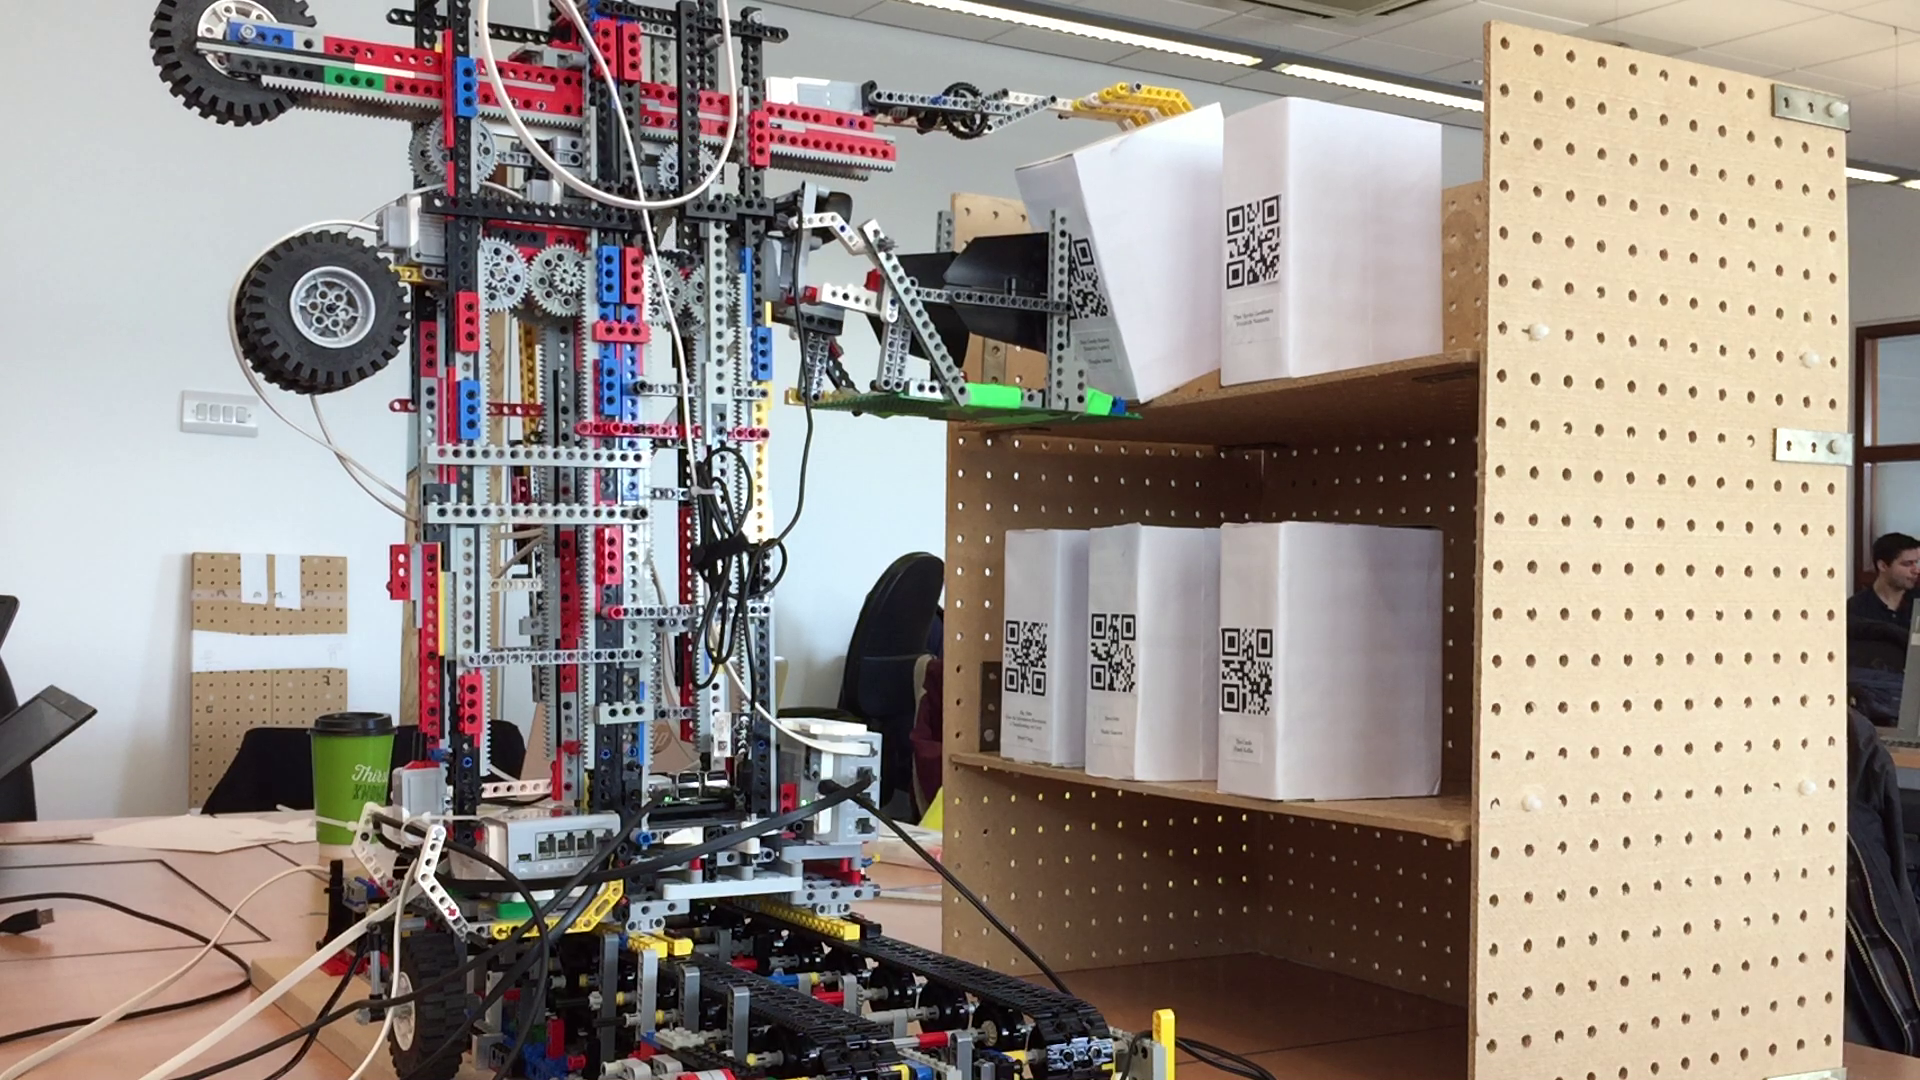
\includegraphics[width=\columnwidth]{figs/crane}}
\caption{Lego construction: highlight any salient features in the caption}
\label{fig:sample-fig}
\end{center}
\vskip -5mm
\end{figure} 

\section*{Submission}
This section is to be deleted.

The document should be submitted on Learn by one group member.

The filename must be  \verb|group-[g]-plan.pdf| where \verb|[g]| is the group number.
This document should be submitted by a group member nominated for this purpose, and also emailed to the group mentor at the time of submission.

%% Include any references in a bibliography

\bibliography{example-refs}

\end{document} 

